\chapter{Warmer and longer growing seasons increase growth for juvenile trees in a common garden}
\label{ch:Wildchrokie}
% \SweaveOpts{concordance=TRUE}


% Set Wildchrokie species shortcut
\newcommand{\Ainc}{\textit{A. incana}}
\newcommand{\Ball}{\textit{B. alleghaniensis}}
\newcommand{\Bpap}{\textit{B. papyrifera}}
\newcommand{\Bpop}{\textit{B. populifolia}}

% \setcounter{secnumdepth}{0} 

% <><><><><><><><><><><><><><><><><><><><><><><><><><><><><><><><><><><><><><><>
% INTRODUCTION
% <><><><><><><><><><><><><><><><><><><><><><><><><><><><><><><><><><><><><><><>
\section{Introduction}

% Paragraph 1
The most frequently observed biological impact of climate change is shifts in phenology---the timing of recurring life history events \citep{parmesan_poleward_1999, menzel_european_2006, calvin_ipcc_2023}. Across many plant species, spring events have advanced \citep{wolfe_climate_2005,chmielewski_response_2001,fu_recent_2014}, while autumn events have delayed---but to a much lesser extent \citep{gallinat_autumn_2015,jeong_macroscale_2014}. Together, early springs and later autumns lengthen the growing season, which should increase growth for many species, including trees \citep{keenan_net_2014, stridbeck_partly_2022}. 

% Paragraph 2
How much trees increase growth with longer seasons is important given the major role of forests in carbon sequestration \citep{friedlingstein_global_2026}. Temperate forests account for roughly 40\% of the annual global carbon sink, diminishing the consequences of human-emitted greenhouse gas emissions on the climate \citep{gibbs_revised_2025}. With warming, research has repeatedly found a connection between longer seasons and increased carbon storage \citep{boisvenue_impacts_2006,gaoEarlierStartThermal2022,finziCarbonBudgetHarvard2020}. The future of this net carbon sink by temperate forests, however, relies on the assumption that longer and warmer seasons will keep increasing carbon storage by trees \citep{pan_enduring_2024}. A shift in this relationship could impact the future of this critical carbon sink.

% Paragraph 3
New studies suggest that longer growing seasons do not always increase growth \citep{dow_warm_2022,silvestro_longer_2023,matula_shifts_2023,charletdesauvage_temperature_2022,cabon_crossbiome_2022}. Recently, \cite{dow_warm_2022} found that warmer springs lengthened the growing season, but did not increase the peak growth rate or total annual growth in two temperate forest communities. Working across biomes, \cite{cabon_crossbiome_2022} found a similar trend, where gross primary production and growth appeared decoupled. However, neither of these studies could clearly establish why they found no relationship, while previous studies have. Understanding whether temperate forests will persist as a net carbon sink requires answering why trees do not grow more despite longer growing seasons. 

% Paragraph 4
A longer growing season does not necessarily mean more favorable thermal conditions for growth. While the well-documented advance of spring phenology elongates the growing season \citep{keenan_net_2014}, spring days are short and usually cool (Figure \ref{fig:GSfig}a). Therefore, this advance may contribute little to a tree's annual growing degree days (GDD) accumulation (Figure \ref{fig:GSfig}b). In contrast, even small shifts to later end of season events can lead to larger changes in annual GDD; since more GDD accumulates per day during this period, any extra end of season days may be more important than additional start of season days \citep{buonaiuto_early_2026}.  

% Paragraph 5
Other factors beyond the thermal conditions may affect whether longer seasons increase growth. While trees may have a longer period to grow, water availability may become insufficient to support continuous growth throughout the growing season \citep{wang_seasonal_2025}. Competition for light and nutrients may further limit the capacity of trees to benefit from longer seasons, especially for the ones positioned below the forest canopy \citep{cleland_effects_2024,augspurger_differences_2003,sweeneyComparisonTimingSpring2024}. Additionally, trees may have internal constraints that prevent them from increasing their growth with longer seasons. Growth, like other biological processes, is under strict genetic control. Thus, even with optimal environmental conditions, physiological constraints may prevent temperate trees from growing indefinitely \citep{korner_four_2023,wolkovich_why_2025}, but we currently have a limited understanding of how well tree phenology and growth can track changing conditions. 

% Paragraph 6
Current research suggests that leaf and wood phenology differ in their plasticity in response to changing environmental conditions across species and life stages \citep{dox_wood_2022}. Leaf phenology (e.g. leafout) in the spring is a highly plastic trait with substantial variation across years with different weather, and also across species. Within a single community leafout can vary across species by over a month, with a general trend of evergreen trees and species with more conservative growth strategies leafing out later \citep{loughnan_budburst_2025}. Additionally, leaf phenology and growth appear closely synchronized in diffuse-porous species \citep[e.g., \textit{Betula;}][]{cufar_treering_2008} and less so in ring-porous species \citep[e.g., \textit{Oaks};][]{gonzalez-gonzalez_comparative_2013}, making leaf phenology a good proxy for setting the start and end of the growing season in angiosperm diffuse-porous species \citep{marchand_timing_2021,silvestro_roots_2025,suzuki_phenological_1996}. While this proxy is useful for setting the boundaries of the growing season, it does not indicate how much trees grow annually. How flexible growth is in response to changing growing season length and conditions varies between species and populations, and may also differ with tree age, with juvenile trees being generally more flexible and responsive than their adult forms \citep{augspurger_differences_2003,way_photoperiod_2015}. 

% Paragraph 7 
Local adaptation could limit tree growth responses of different populations to future climate \citep{soolanayakanahally_timing_2013,wolkovich_why_2025}. While leaf phenology (e.g. leafout) in the spring is highly plastic and driven by temperature, end of season phenology (e.g. budset) is much less plastic and mostly driven by photoperiod \citep{baumgarten_indeterminacy_2026,singh_photoperiod_2017}, with evidence of local adaptation \citep{zeng_weak_2024}. Provenance trials have repeatedly found trees from northern latitudes set bud earlier, even when grown in warm climates with longer growing seasons \citep{aitken_time_2016,way_photoperiod_2015}. This local adaptation and related reliance on photoperiod to trigger budset (an end of season event) likely explain why shifts in EOS with warming have been so much smaller than shifts in start of season. This predicts a latitudinal gradient in growth responses, with more limited responses in poleward populations where the end of season is constrained to happen earlier in the season. Thus, common gardens investigating the effect of provenance latitude could help predict how climate change will affect tree growth. 

% Paragraph 8
To understand the relationship between growing seasons and growth, we need to understand how growth varies across species and populations while disentangling how much longer seasons are also more thermally favorable seasons. Here, we address this by studying how growth and growing seasons relate across species, populations and multiple metrics of growing season length. Working with four juvenile tree species sourced from four populations and grown in one common garden, we examine how growth, measured via tree rings, and leaf phenology covary over three years. We consider effects of both the length of the season (i.e. number of growing days in the season) and its thermal conditions (i.e. GDD accumulated in the season). 

% Conceptual figure
\begin{figure}[!ht]
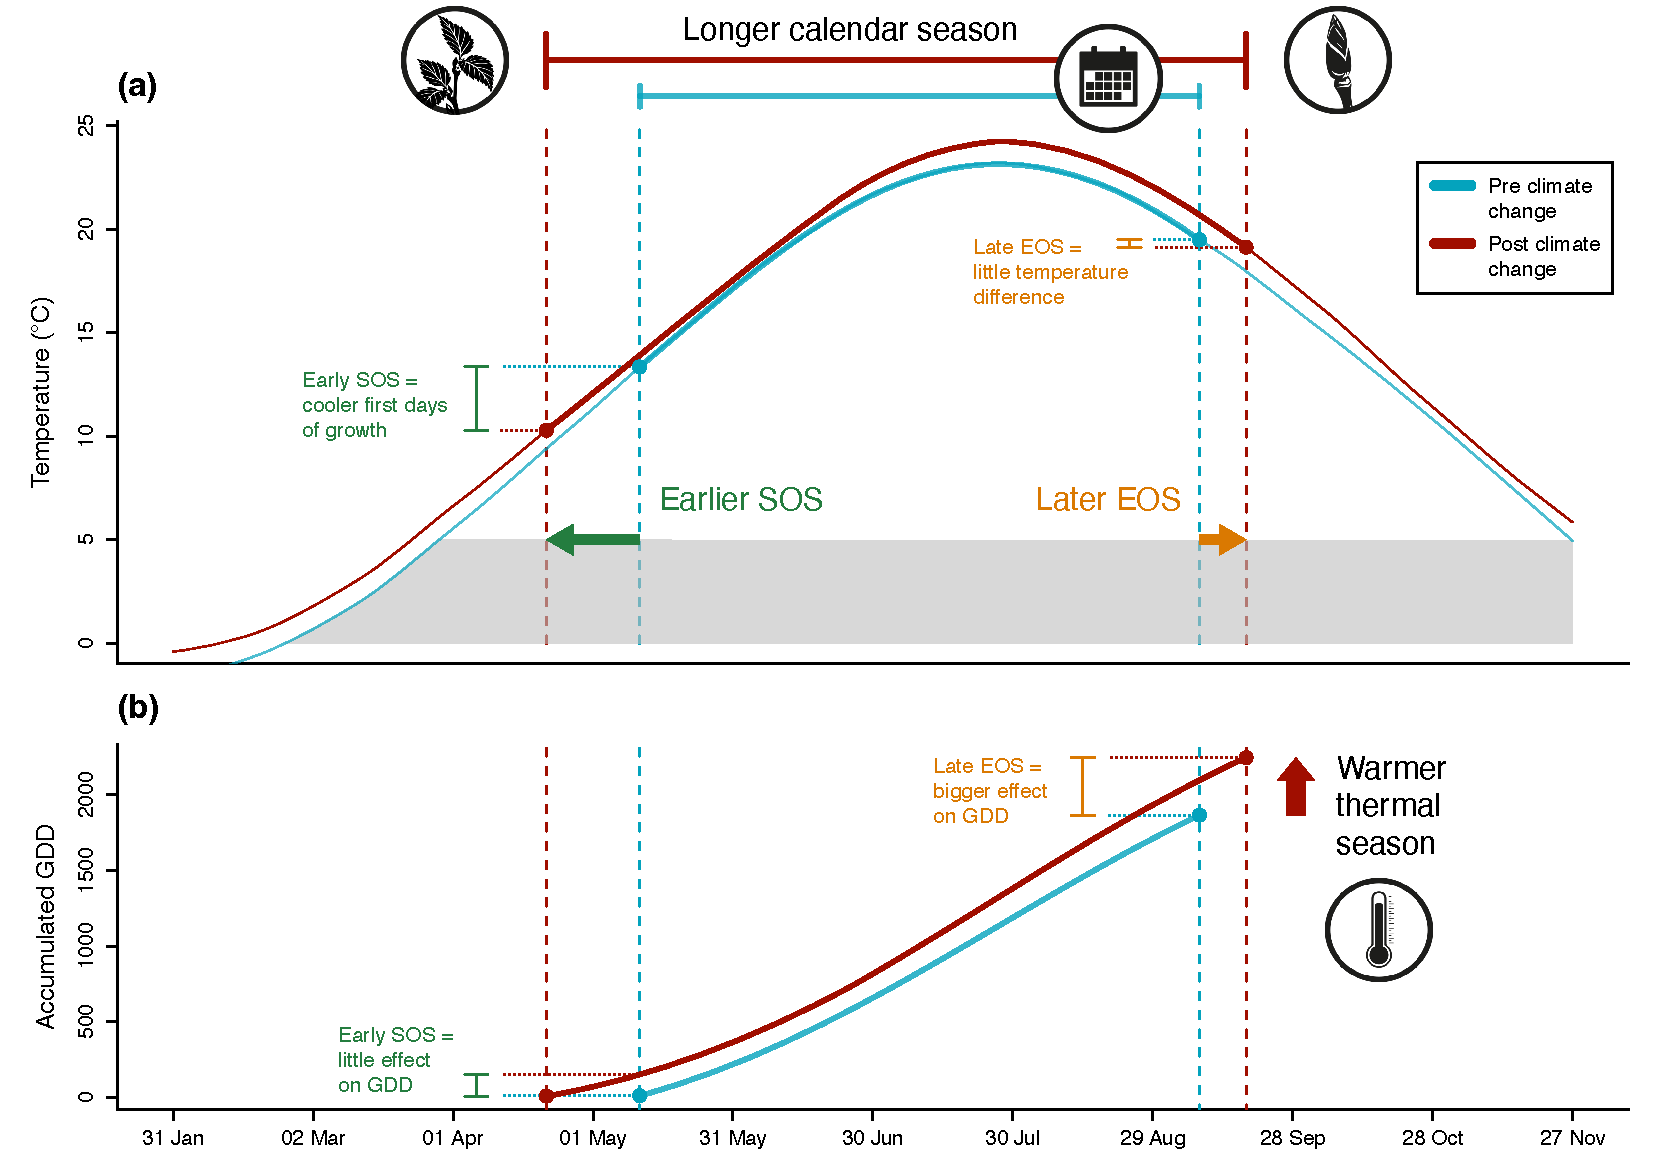
\includegraphics[width=0.9\textwidth]{../figures/wildchrokie/climate/gsconceptualfig.pdf}
\caption{Shifting growing season lengths with climate change affects both the temperature trees experience throughout the growing season (a) and how many growing degree days (GDD) they accumulate (b). Here we show changes in daily (smoothed) and accumulated temperatures before (1945-1965, in blue) and significant anthropogenic climate warming (2005-2025, in red) using data local to our study. The arrows represent hypothetical shifts in spring (green) and fall (orange) phenology. With climate change, spring events have advanced and fall phenology has delayed, but to a much lesser extent---lengthening the calendar growing season. This concurrently changed the temperature trees experience early in their season, with cooler first days of growth (a) causing little accumulation of GDD (b). In contrast, weaker shifts in end of season and little temperature change (a) result in a relatively high GDD accumulation (b) due to warmer temperatures at this time of the season. Alongside these start and end of season shifts, warmer summer temperatures increased GDD accumulation, further warming their thermal seasons. We used mean daily temperature data from the Boston Logan International Airport Climate station for the smoothed temperature and GDD curves \citep{nationaloceanicandatmosphericadministration_local_2026}. }
\label{fig:GSfig}
\end{figure}

% <><><><><><><><><><><><><><><><><><><><><><><><><><><><><><><><><><><><><><><>
% METHODS
% <><><><><><><><><><><><><><><><><><><><><><><><><><><><><><><><><><><><><><><>
\clearpage
\section{Materials and Methods}

%-------------------------------------------------------------------------------
% Common garden setup
%-------------------------------------------------------------------------------
\subsection{Common garden setup and data collection}
We collected seeds from 18 species of deciduous trees and shrubs from four provenances across a 3.5$^{\circ}$ latitudinal gradient (Figure \ref{fig:mapProv}; Table \ref{tab:tab_species}, \ref{tab:climate}) in 2014-2015, germinated them following standard germination protocols and grew them to seedlings \citep{baskin_seeds_2014}. In the spring of 2017, we planted the seedlings outside at the Weld Hill Research Building at the Arnold Arboretum in Boston MA (42.30\degree N, 71.13\degree W). Plots were regularly weeded and watered throughout the duration of the study and were pruned for airflow approximately 1.5 meters above the ground in the fall of 2020 \citep{buonaiuto_early_2026}. 

For the years 2018-2020, we monitored leaf phenology for all individuals in the common garden once or twice per week from February to December; the exact frequency varied within and across years (for more details, see Figure \ref{fig:phenoTimeSeries}). For this, we used a modified BBCH scale to observe two phenological stages: leafout, which we defined as: BBCH 15 and budset as BBCH 102 \citep[proposed phenophases in][]{finn_general_2007,buonaiuto_early_2026}. We had a total of 239 leafout and 230 budset observations (which we refer to as the `full datasets'), but for some individual trees in certain years we did not have both events; thus our total of matched full growing season duration (which we refer to as the `restricted dataset') is 227 observations across 81 individuals.  

In the spring of 2023, we collected tree ring samples from tree species with high survivorship. Thus, we have four species in the \textit{Betulaceae} family: grey alder (\textit{Alnus incana}), yellow birch (\textit{Betula alleghaniensis}), paper birch (\textit{Betula papyrifera}) and grey birch (\textit{Betula populifolia}). We collected cross-sections on 78 individuals by cutting the trunk 2 cm above the root collar, and cores on 43 individuals using standard dendrochronological methods \citep{cook_methods_1990}, for a total of 81 individual trees (Table \ref{tab:tab_species}). We stored the cores in modified (with holes) plastic straws to promote aeration and left them to dry with the cross-sections at ambient temperature for three months. 

% Provenance map
\begin{figure}[!ht]

\includegraphics[width=0.9\textwidth]{/Users/christophe_rouleau-desrochers/github/wildchrokie/analyses/figures/empiricalData/mapSourcePop.pdf}
\caption{Provenances where the seeds were sourced from are depicted as circles, while the diamond denotes the location of the common garden. The common garden location is where the study took place at the Weld Research Building (Boston, MA). The colors of the dots match the model estimates of Figure \ref{fig:wcmuplotasite}. 
We provide climate variables in Table \ref{tab:tab_species}.}
\label{fig:mapProv}
\end{figure}

%-------------------------------------------------------------------------------
% Sample processing, imaging and measuring
%-------------------------------------------------------------------------------
\subsection{Sample processing, imaging and measuring}
We mounted cores on wooden mounts, and sanded both the cores and cross-sections using progressively finer sandpaper grits (150, 300, 400, 600, 800, 1000), then scanned the cores and cross-sections at a resolution of 6250 dpi with a high-resolution tree ring scanner \citep{fong_tim_2026}. Using the digitized images, we measured ring widths with ImageJ \citep{schneider_nih_2012} at three standard locations for each cross-section (at {120\degree} from each other, averaging the three measurements to yield one ring width per year, per individual), and one ring width for each core. Since trees do not grow symmetrically, having three measurements at different angles is better than one. Therefore, when we had cross-sections ($n = 78$) and cores ($n = 43$) for an individual, we used only the measurements from the cross sections ($n = 81 $).

We performed visual cross-dating. This consists of assigning a calendar year to each ring and comparing the year-to-year growth variation and anomalies across replicates of the same species \citep{cook_methods_1990}. We did not perform statistical crossdating or detrending because our chronologies (number of years of data) were extremely short \citep{radenPotentialIntraannualDensity2020a} and showed no evidence of consistent allometric trends (Figure \ref{fig:allom}). We controlled for effects of different years by including `year' in our models (see equation \ref{eq:mainMdl} in `Data analyses' below).

\subsection{Data analyses}
To understand how growth shifted with season length, we used Bayesian hierarchical models, estimating how growth, measured as ring width, covaried with season length, measured in four different ways: GDD, GSL, SOS and EOS. We calculated the thermal season using growing degree days (GDD; mean daily temperature above 5\degree C) accumulated between leafout and budset, and the calendar season (or growing season length; GSL) as the number of days between leafout and budset. Finally, we used leafout as the start (SOS) and budset end of the season (EOS) as separate predictors that represent the boundaries of the growing season. For interpretability, we report ring width change (log(mm)) per GDDs accumulated in an average week (seven days) in May (day of year 121 to 150 from 2018 to 2020), for the thermal season, and ring width change per week of season length, leafout and budset for GSL, SOS and EOS, respectively. We report effects when the 90\% uncertainty intervals (UI) do not overlap with zero and consider a trend if the 50\% UI do not overlap with zero.

For daily climate data across all the years of phenological sampling (2018-2020), we combined two sources. For 2018 and 2019, we used data from the climate station located at Weld Hill research station \citep{arnoldarboretum_weather_2026}. Because the data were not available for that station after August 2020, we used data from the weather station `Boston (Weld Hill)' of the Network for Environment and Weather Applications (NEWA) for the whole year in 2020 \citep[see Figure \ref{fig:climOverlap} for the climate overlap between the two stations in 2020;][]{carroll_network_2026}. We used the North American Drought Monitor Maps to determine drought occurrence across years at our study location and used the proposed drought intensity index to qualify the presence of moderate, severe or extreme droughts \citep{nationalcentersforenvironmentalinformationncei_north_2026}. 

For each predictor, we estimated its effect on observed ring width ($i$, denoting each observation) for each tree ($treeid$) in each year ($year$) as:

\begin{equation}
\begin{aligned} 
ln(ringwidth)_i &\sim Normal(\mu, \sigma_y) \\
\mu &= \alpha + \alpha_{\text{species}} + \alpha_{\text{prov}} + \alpha_{\text{treeid}} + \alpha_{\text{year}} + \beta_{species} \times \text{season predictor} \\
\alpha_{\text{prov}} &\sim Normal(0, \sigma_{\alpha \, \text{prov}}) \\
\alpha_{\text{treeid}} &\sim Normal(0, \sigma_{\alpha \, \text{treeid}}) \\
\end{aligned}
\label{eq:mainMdl}
\end{equation}

This model estimates a species-specific effect of each season length predictor (e.g. GDD) on growth ($\beta_{species}$), while also controlling for other variation due to species ($\alpha_{species}$), provenance ($\alpha_{prov}$), individual tree ($\alpha_{treeid}$) and year ($\alpha_{year}$). We ran the models using both natural units, and also using scaled predictors \citep[via $z$-scoring;][]{gelman_data_2006} to allow for direct comparison of effect sizes across different metrics. We report estimates as means and 90\% uncertainty intervals (UI).  

We used weakly informative priors for all models (increasing the priors by 2$\times$ for the $z$-scored models did not qualitatively affect the results). We ran four chains with 2000 warm-up and 2000 sampling iterations each, for a total of 8000 sampling iterations and checked diagnostics of output: chains had no divergent transitions, $\hat{R}$ values below 1.01, and effective sample sizes ($n_{\text{eff}}$) greater than 10\% of the model iterations. We also fit the models for SOS and EOS using both the restricted ($n =$ 227) and full datasets for each predictor (SOS $n =$ 239 and EOS $n =$ 230. We wrote our models using Stan \citep{carpenter_stan_2017} with the rstan package version 2.32.7 \citep{standevelopmentteam_rstan_2025} to run the Stan code in R. 

Because ring widths decrease with age---particularly with young trees---we also ran the models using basal area increment as the response variable only for the 78 replicates with cross-sections. This allows for a more representative portrayal of annual growth increment by using the total ring area, instead of its width alone. To calculate basal area increment, we summed each ring width separately at the three distinct locations on the cross sections, yielding three radii from pit to bark. We then calculated the area of each ring by subtracting the radius from the inner ring from the outer ring: $\pi \times (\text{inner radius}^2 - \text{outer radius}^2)$, and averaged across the three BAI for each ring. 


% <><><><><><><><><><><><><><><><><><><><><><><><><><><><><><><><><><><><><><><>
% RESULTS
% <><><><><><><><><><><><><><><><><><><><><><><><><><><><><><><><><><><><><><><>
% \clearpage
\section{Results}
%-------------------------------------------------------------------------------
% Info
%-------------------------------------------------------------------------------
At the common garden location, the mean summer temperature was similar across years, with 2019 being the coolest 
(22.38$^\circ$C), 2020 the hottest 
(23.07$^\circ$C), and 2018 in between 
(22.85$^\circ$C). There was no drought for those three years, except for in 2020, when a moderate summer drought (June-August) ramped up to a severe drought in September \citep{nationalcentersforenvironmentalinformationncei_north_2026}.
The calendar and thermal seasons ranged from 
90 days and 
1465.1 GDD ({\Ball} in 2018) to 
173 days and 2513.6 GDD ({\Ainc} in 2018; Figure \ref{fig:wcboxplotPred}a and b). 
The earliest leafout was
22-Apr ({\Ainc} in
2019) and the latest,
05-Jun (also {\Ainc}, but in
2020; Figure \ref{fig:wcboxplotPred}c). The earliest budset was 
13-Aug ({\Ball} in
2018) and the latest, 
24-Oct ({\Ainc} in
2018; Figure \ref{fig:wcboxplotPred}d). Finally, annual ring widths across years varied from 
0.39 mm ({\Ball} in 2020) to 
13.55 mm ({\Bpop} in 2018; Figure \ref{fig:wcboxplotRW}).  


%-------------------------------------------------------------------------------
% Question 1
%-------------------------------------------------------------------------------
Longer growing seasons increased growth for all species, but varied depending on the metric used to measure it. We report estimates as means and 90\% uncertainty intervals (UI) that correspond to ring width change in \% ---henceforth `\%/day'  or `\%/GDD,' with days and GDD being adjusted to represent more meaningful units, as described above (see `Data analyses' section in Methods for more details).
Warmer thermal seasons increased growth for paper birch (\textit{Betula papyrifera}; $\beta =$
16.05, UI:
6.37, 
26.05 \%/GDD), grey birch (\textit{Betula populifolia}; $\beta =$
7.23, UI: 
2.33, 
12.25 \%/GDD), and yellow birch (\textit{Betula alleghaniensis}; $\beta =$
4.22, UI: 
0.45, 
8.15 \%/GDD), grey alder (\textit{Alnus incana}) trended in the same direction ($\beta =$ 
2.18, UI: 
-1.1, 
5.57 \%/GDD); Figure \ref{fig:wcmuplotbspp}a and e; Table\ref{tab:wc_slope_table}).
Unlike its response to warmer thermal season, {\Ainc} grew more with longer calendar seasons ($\beta =$
5.27, UI: 
0.14,
10.66 \%/day). {\Bpap} also grew more with longer calendar seasons
($\beta =$ 20.7, UI: 
5.39, 
37.14 \%/day), while the other two \textit{Betula} did not, though they trended in the same way ({\Ball}: $\beta =$
3.39, UI: 
-2.69, 
9.74 \%/day, and {\Bpop}: $\beta =$
5.87, UI: 
-1.91, 
13.99 \%/day; Figure \ref{fig:wcmuplotbspp}b and f; Table \ref{tab:wc_slope_table}). 
On a scaled axis \citep[through $z$-scoring,][]{gelman_data_2006}, the thermal and calendar seasons were similarly predictive (Figure \ref{fig:bsppZscored}). Results with basal area increment (BAI) for the GDD model were similar to ring width (see Table \ref{tab:BAItab}). 


%-------------------------------------------------------------------------------
% Question 2
%-------------------------------------------------------------------------------
In contrast to our expectation, we found most species grew more with a later end of season, and only one species grew more with an earlier start of season ({\Ainc} (one of the two species that a longer calendar season increased growth for: $\beta =$
-7.07, UI:
-12.73, 
-1.14 \%/day; Figure \ref{fig:wcmuplotbspp}c and g; Table \ref{tab:wc_slope_table}). 
{\Bpop} trended in the opposite direction ($\beta =$
5.05, UI:
-6.93, 
17.84 \%/day; Figure \ref{fig:wcmuplotbspp}c and g; Table \ref{tab:wc_slope_table}). {\Ball}, which did not grow more with longer calendar season, grew less with an earlier start of season ($\beta =$
10.65, UI:
0.48, 
21.60 \%/day; Figure \ref{fig:wcmuplotbspp}c and g; Table \ref{tab:wc_slope_table})---but more with a later end of season ($\beta =$ 
12.22, UI:
5, 
19.68 \%/day). Alongside {\Ball}, two other species grew more with a later end of season ({\Bpop}: $\beta =$
10.17, UI:
2.65, 
18.03 \%/day, and {\Bpap}: $\beta =$
23.58, UI:
9.28, 
39.01 \%/day; Figure \ref{fig:wcmuplotbspp}d and h; Table \ref{tab:wc_slope_table}), with the latter being the only one of those three that also grew more with longer calendar season. The estimates were unchanged when using the full (SOS: $n =$
239 and EOS: $n =$
230) or restricted datasets ($n =$ 
227; Figure \ref{fig:wcSOSEOScomparison}a). 


%-------------------------------------------------------------------------------
% Question 3
%-------------------------------------------------------------------------------
We did not find any clear effect of year on growth (2018: $\alpha =$
0.19, UI:
-0.77, 
1.15 RW; 2019: $\alpha =$
0.18, UI:
-0.79, 
1.14 RW; 2020: $\alpha =$
-0.43, UI:
-1.40, 
0.53 RW; Table \ref{tab:tab_all}), and there were no apparent differences in baseline growth between species ({\Ainc}: $\alpha =$
1.06, UI:
-3.19, 
5.21 RW; {\Ball}: $\alpha =$
0.21, UI:
-3.97, 
4.34 RW; {\Bpap}: $\alpha =$
-4.00, UI:
-8.89, 
0.75 RW; {\Bpop}: $\alpha =$
-0.66, UI:
-4.94, 
3.63 RW; Figure \ref{fig:wcxyGDD} and \ref{fig:wcxyGSL}; Table \ref{tab:tab_all}). In addition, growth did not vary with provenance (Dartmouth College (NH): $\alpha =$
-0.03, UI:
-0.22, 
0.14 RW; Harvard Forest (MA): $\alpha =$
-0.10, UI:
-0.33, 
0.07 RW; St-Hippolyte (Qc): $\alpha =$
0.04, UI:
-0.14, 
0.24 RW; White Mountains (NH): $\alpha =$
0.08, UI:
-0.09, 
0.29 RW; Figure \ref{fig:wcmuplotasite}; Table \ref{tab:wc_asite_table}). The estimates did not change when fitting the species provenances individually (see Figure \ref{fig:wcmuplotasitePerSpp} for details on this separate intercept-only model). The limited variation between provenances ($\sigma = $
0.17, UI:
0.02, 
0.48 RW) was similar to variation across individual trees ($\sigma =$ 
0.17, UI: 
0.05, 
0.27 RW; Table \ref{tab:tab_all}).


% Figure mu across all species and climate predictors
\begin{figure}[!ht]
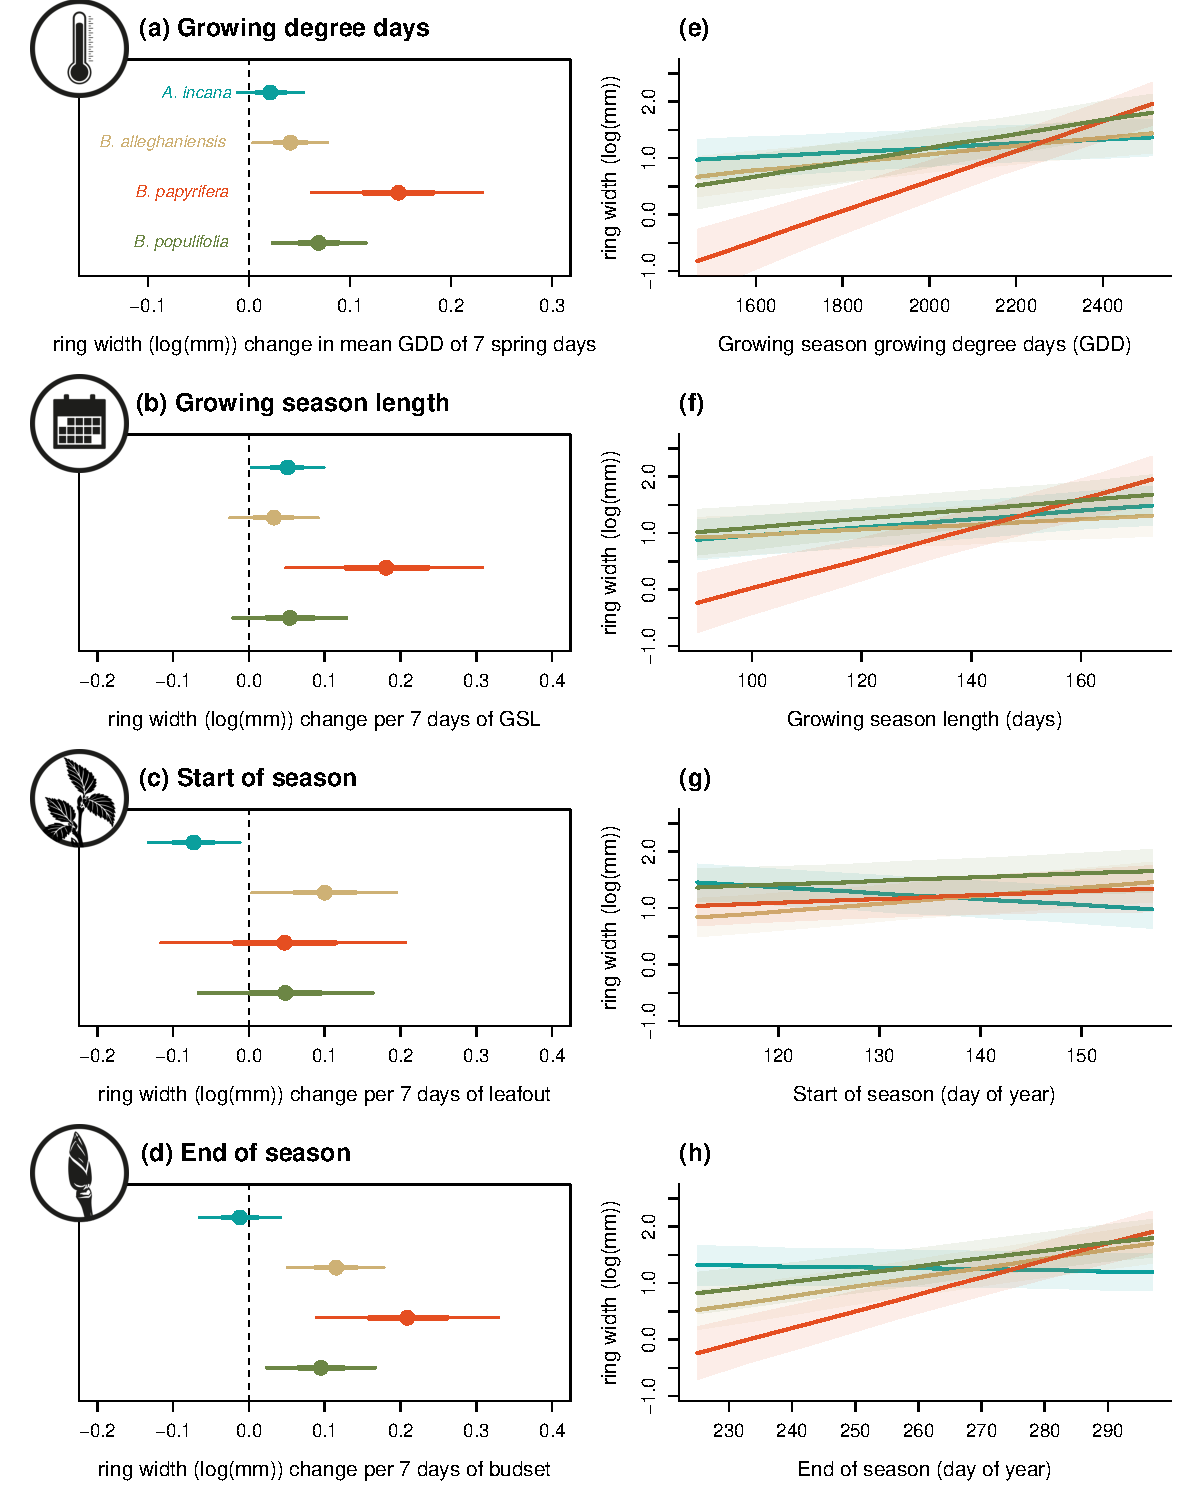
\includegraphics[width=0.8\textwidth]{../figures/wildchrokie/growthModelsMain/muALLbsppWlines.pdf}
\caption{Estimates of ring width change (log(mm)) as a function of four different phenological predictors: growing degree days of the growing season (mean daily temperature above 5\degree C); growing season length, start of season, and end of season across four species: grey alder (\textit{Alnus incana}), yellow birch (\textit{Betula alleghaniensis}), paper birch (\textit{Betula papyrifera}) and grey birch (\textit{Betula populifolia}; species colors are the same across the panels). Panels on the left (a to d) represent the mean model slope estimates for each species (dots) with 50\% and 90\% uncertainty intervals (thicker and thinner lines, respectively), for each predictor, which we represent through ring width change in mm on the log scale per adjusted predictor (see `Data analyses' section in Methods for more details on predictor adjustment). See Table \ref{tab:wc_slope_table} for parameter estimates. Panels on the right (e to h) show the estimated response of ring width as a function of each predictor, with the lines depicting the mean response at each predictor value, and the shaded area, the 50\% uncertainty intervals.}
\label{fig:wcmuplotbspp}
\end{figure}



% <><><><><><><><><><><><><><><><><><><><><><><><><><><><><><><><><><><><><><><>
% DISCUSSION
% <><><><><><><><><><><><><><><><><><><><><><><><><><><><><><><><><><><><><><><>
\clearpage
\section{Discussion}
Here we used 81 juvenile trees of four species from four provenances to study how longer growing seasons affect tree growth (using annual growth via tree rings and leaf phenology as a proxy for the start and end of season). Longer growing season increased growth for all species, but varied depending on the metric used to measure season length, with the thermal growing season more often relating to growth than the calendar season.

Our results support the idea that the thermal season is a better predictor for growth \citep{chuine_processbased_2017,wang_simulation_1998}. By accounting for differences in daily temperatures, the thermal season may be more closely aligned with when and how fast plants can grow each day compared to the calendar season, which assumes a stable influence of each day on growth. Thus, the short and cool spring days early in the season count for less in the thermal season than the calendar season \citep{buonaiuto_early_2026}. Further supporting this, when we disentangled the calendar season by using the start and end of season separately, we found a larger response of growth to the end of season, with little effect of the start of season. 

The finding that the end of season appears more related to growth than the start of season is aligned with increasing work suggesting the start and end of season together may dynamically determine growth \citep{zohner_effect_2023}. This implies that research focusing solely on start of season \citep{dow_warm_2022,gaoEarlierStartThermal2022,wheeler_snow_2016} could miss when longer seasons lead to more growth, and also that the strong focus on start of season in phenology research may ignore an important part of the season for growth. While studies have long called for more research on the end of season \citep{gallinat_autumn_2015,gunderson_forest_2012,piao_plant_2019,richardson_terrestrial_2012}, our results suggest we may especially need more work that monitors how growth and phenology shift across the season \citep{zani_increased_2020,zohner_effect_2023}. More studies using data with a finer temporal scale (e.g., daily or weekly data through dendrometers and/or xylogenesis) could confirm whether most growth occurs closer to the end of season versus the start of season. To date, these studies have shown strong species differences as to when most of the growth happens in the season. However, most of these studies were done on a small number of European and/or conifer species \citep[e.g.][]{zweifel_are_2016,etzold_number_2022,balducci_stem_2019}. More data across species spanning a wider range of life history strategies could elucidate how dynamically growth can change throughout the season.

Our results suggest that different growth strategies between species may yield different responses to longer seasons. Our most ruderal species, {\Ainc} was the only species to grow more with a longer calendar season and an earlier start of season\citep{grime_evidence_1977}. This suggests that species with more ruderal, flexible life-history strategies may actually take advantage of growing more in the spring despite cooler, shorter days \citep{bowmanEcology2023,furlow_alnus_1997,grime_evidence_1977}. In contrast, {\Bpap} and {\Bpop}, which are fast growing, but more conservative than {\Ainc}, were both most driven by the end of season, suggesting that they would be able to exploit these late season days characterized by warmer temperatures \citep{burns_silvics_1990}. Lastly, our slowest growing, longest living species, {\Ball}, responded to both the start and end of season. This points towards a possible `neutralizing' response where an early start of season decreases growth, but a later end of season increases it, muting this species' response to a longer calendar season. Studies including an even wider span of growth strategies across species may find further differences. Our four study species all grow under closed canopy are relatively fast-growing, which should allow them to track changing conditions better than their slower-growing counterparts. While we found an overall positive trend of warmer seasons on growth, this might have changed if we used slower growing, more conservative species \citep[such as \textit{Quercus};][]{burns_silvics_1990}. Additionally, we used juvenile trees, which tend to be more reactive and could in part explain why they grew more with warmer seasons \citep{augspurger_differences_2003,sweeneyComparisonTimingSpring2024}. While other studies on mature trees have found the same result, our results may have been more muted if the trees were grown in a forest setting. We grew trees in a common garden setting with potentially more space between trees than in a natural setting (spacing was between 1.5 and 3 m), without any shade cloth. If these trees grew in a mature forest, they would have been below the canopy, competing for light and other resources and thus might not have responded as much as we observed in our competition-limited conditions \citep{polgar_leafout_2011}. However, our results may have implications beyond how mature forests function. 

Our focus on juvenile trees may suggest how forests regenerate and assemble with the longer, warmer seasons of anthropogenic climate change. Plant phenology research has suggested that earlier seasons with warming favor the species that shift earlier the most, with many studies focused on invasive species appearing to support this \citep{wolkovich_temperaturedependent_2013,zettlemoyer_phenology_2019}. Yet, these studies are often on herbaceous species, and our results, along with other recent work \citep{zani_increased_2020,zohner_effect_2023}, suggest mid- and later-season effects may have underappreciated performance implications in woody species. Thus, more studies of how later-season events correlate with invasions, and forest assembly more generally, could be especially important for understanding how warming will shift forest regeneration.

Our results also suggest that population-level differences in assembly models may not be as critical as previously suggested \citep{cavender-bares_diversification_2019}. While studies of large latitudinal gradients have found lower growth in tree species from poleward latitudes \citep{soolanayakanahally_timing_2013,aitken_time_2016}, we found little difference in growth across a latitudinal gradient of 3.5\degree. Thus, at least across this latitudinal range, local adaptation on growth for these species appears weak. Supporting this, we found no evidence of shifting end of season across provenances in these four closely related species, on average, despite decades of work finding that end of season events, such as budset, are usually more locally adapted than start of season events such as leafout \citep{kramer_effect_1936,habjorg_photoperiodic_1978,keller_climatedriven_2011,soolanayakanahally_timing_2013,aitken_time_2016,zeng_weak_2024}. Yet, a study of the same common garden, including all tree and shrub species found end of season appeared to vary strongly by year and shift earlier with earlier start of season \citep{buonaiuto_early_2026}, suggesting end of season may be more variable than currently proposed \citep{alberto_potential_2013}. However, compared to other studies that found strong local adaptation on growth and budset \citep[e.g.][]{rohde_bud_2011}, we had little replication per species across a smaller latitudinal gradient. Taken together, these results imply that our current understanding of budset being strongly locally adapted and thus varying little with temperature or start of season needs more study. 

\subsection{Implications for large-scale vegetation modeling}
Using a rarely available dataset of tree growth coupled with leaf phenology start and end season, we found an overall positive response from multiple tree species to longer seasons, which has important implications for models of future carbon storage. While juvenile trees store little carbon compared to their adult forms, they are crucial for forest regeneration capacity and range expansion \citep[as discussed above, and see][]{luu_importance_2024}, and generally predict adult tree responses qualitatively \citep{wolkovich_why_2025}. We found that the start and end of season asymmetrically matter to growth, which means that how we model these phenological events in vegetation and related earth system models may be critical for accurate predictions. Modelling the end of season better will require more studies, especially on more species across a larger gradient. This could help tease out whether local adaptation of end of season depends on the species, latitudinal range (both distance and how far north provenances come from), or some combination of the two, which could then feed into improved models. 

Integrating our results into models will also require considering how environmental conditions beyond temperature shift across the season, especially soil moisture \citep{gaoEarlierStartThermal2022,li_widespread_2023}. Trees in our common garden were regularly watered, likely relieving any major drought pressures, though studies beyond ours have found a connection between a later the end of season and more growth, \citep[see:][]{gaoEarlierStartThermal2022,wang_seasonal_2025}. For the four species we studied, there are currently no increases in drought occurrence within their ranges \citep{nationalcentersforenvironmentalinformationncei_north_2026,agel_drought_2025}, suggesting that their growth may increase with longer and warmer growing seasons \citep{cook_uncertainty_2011,agel_drought_2025}, as we found. However, the positive effect of a later end of season could be offset if soil moisture becomes inadequate for growth, and other temperate regions with decreased soil moisture have reported declines in tree growth \citep[e.g.,][]{chiang_evidence_2021,spinoni_will_2018}. Improved accuracy of future carbon sequestration models would consequently require integrating over more regions and growth drivers.


